\documentclass[hidelinks,12pt]{article}

% ==============================
% Essential Packages
% ==============================
\usepackage[utf8]{inputenc}
\usepackage[margin=2.5cm]{geometry}
\usepackage{amsmath, amssymb, mathtools, bm}
\usepackage{graphicx}
\usepackage{hhline}
\usepackage{mathdots}
\usepackage{color}
\usepackage{tikz}
\usepackage{fancyhdr}
\usepackage{enumitem}
\usepackage{lmodern}
\usepackage{pdflscape}
\usepackage{esvect}
\usepackage{centernot}
\usepackage[driverfallback=hypertex]{hyperref}

% ==============================
% Page Layout
% ==============================
\setlength{\parindent}{1cm}
\newgeometry{left=2cm, right=2cm, top=2.5cm, bottom=2.5cm}

% ==============================
% Header and Footer
% ==============================
\pagestyle{fancy}
\fancyhf{}
\fancyhead[LE,RO]{Page \thepage\ of 32}
\fancyhead[RE,LO]{\leftmark}
\fancyfoot[CE,CO]{Fiedler’s Theory of Spectral Graph Partitioning}
\renewcommand{\headrulewidth}{2pt}
\renewcommand{\footrulewidth}{1pt}

% ==============================
% Document Starts
% ==============================
\begin{document}

\vspace*{3cm}

% ==============================
% Title Page
% ==============================
\begin{center}
{\fontsize{22pt}{26pt}\selectfont \textbf{\textit{Fiedler’s Theory of Spectral}}\\[0.2cm]
\textbf{\textit{Graph Partitioning}}} \\[2cm]

{\Large 
    Ayushman Anupam (MDS202411)\\
    Biswajit Kala (MDS202412)\\
    Boda Surya Venkata Jyothi Sowmya (MDS202413)
} \\[1cm]

{\large 
    \emph{Supervisor:} Kavita Sutar Deshpande
} \\[1cm]

\Large Data Science \\
Chennai Mathematical Institute \\[2cm]
\end{center}

% ==============================
\newpage
\tableofcontents
\newpage

% ==============================
% Abstract
% ==============================
\section{Abstract}
\noindent
The growing prevalence of graph-structured data in modern applications poses unique challenges in terms of scalability, storage, and analysis. Unlike tabular data, graphs require partitioning strategies that retain structural relationships and connectivity.

\vspace{1em}
\noindent
This report explores \textbf{Fiedler’s Spectral Graph Partitioning} as a principled approach to segmenting large graphs without compromising their intrinsic structure. Rooted in spectral graph theory, the method leverages the Laplacian matrix and its eigenvectors—particularly the Fiedler vector—to identify natural partitions.

\vspace{1em}
\noindent
Key contributions of this work include:
\begin{itemize}
    \item A rigorous mathematical treatment of graph Laplacians and their spectral characteristics
    \item A formal proof of Fiedler’s theorem ensuring connected subgraphs
    \item Strategies for practical and computationally efficient implementation
    \item Empirical validation using synthetic and real-world graph datasets
\end{itemize}

\vspace{1em}
\noindent
Our findings suggest that Fiedler’s method offers a robust and interpretable framework for graph partitioning. It is particularly suited to applications demanding balanced divisions and preserved connectivity, such as parallel computing, social network analysis, and biological systems modeling.

\vspace{1em}
\noindent
This report contributes to the field of graph algorithms by providing both theoretical insights and practical considerations for deploying spectral methods in real-world scenarios.

% ==============================
\newpage
\section{Acknowledgement}

\parbox{0.9\textwidth}{
We express our sincere gratitude to all those who supported and guided us throughout this project.

\vspace{1em}
First and foremost, we are deeply thankful to \textbf{Kavita Sutar Deshpande}, our project guide, for her valuable insights, continuous support, and encouragement.

\vspace{1em}
We also extend our thanks to the faculty and staff of the \textbf{Department of Data Science} at \textbf{Chennai Mathematical Institute}, for providing a conducive environment for research and learning.

\vspace{1em}
We are grateful to our peers and friends for their help, motivation, and meaningful discussions during the project.

\vspace{1em}
Finally, we thank our families for their unwavering support and encouragement throughout our academic journey.
}

\newpage
\section{Introduction}

\subsection*{Background}
Modern data systems increasingly rely on large-scale graph structures, which present significant challenges in storage, computation, and analysis due to their high connectivity. Unlike tabular data, which can be partitioned straightforwardly, graph data requires careful segmentation to preserve essential structural relationships. Spectral graph theory, and in particular Fiedler’s method, offers a mathematically grounded and effective strategy for partitioning such graphs while maintaining their integrity.

\subsection{Problem Statement}
This work focuses on the problem of partitioning a large, connected graph into two smaller subgraphs such that:
\begin{itemize}
    \item The number of edges crossing between the two subgraphs is minimized,
    \item Each resulting subgraph remains internally connected,
    \item The partition is balanced with respect to the number of vertices.
\end{itemize}
This problem is critical in applications such as distributed computing, parallel processing, and social network analysis.

\subsection*{Aim and Objectives}
\textbf{Aim:} To explore and implement Fiedler's Spectral Graph Partitioning method for effective and balanced graph segmentation.

\vspace{0.5em}
\noindent\textbf{Objectives:}
\begin{itemize}
    \item Understand the mathematical foundations of spectral graph theory.
    \item Analyze the properties of the Laplacian matrix and its eigenvectors.
    \item Implement Fiedler’s method and demonstrate it on representative graphs.
    \item Establish that the resulting subgraphs are connected.
    \item Evaluate the performance and potential applications of the method.
\end{itemize}
\newpage

\subsection{Solution Approach}
The solution is based on Fiedler's spectral method, which involves the following steps:
\begin{enumerate}
    \item Construct the Laplacian matrix \( L = D - A \), where \( D \) is the degree matrix and \( A \) is the adjacency matrix.
    \item Compute the eigenvalues and eigenvectors of \( L \).
    \item Use the second-smallest eigenvector (known as the Fiedler vector) to assign vertices to two partitions based on the sign (positive or negative) of their corresponding components.
\end{enumerate}
This approach minimizes edge cuts and promotes connectivity within each subgraph.

\subsection*{Summary of Key Outcomes}
\begin{itemize}
    \item Developed a complete implementation of Fiedler’s spectral partitioning algorithm.
    \item Demonstrated that the method yields connected and relatively balanced subgraphs.
    \item Validated theoretical claims using controlled examples with small graphs.
    \item Discussed the advantages, limitations, and practical relevance of the method in real-world scenarios.
\end{itemize}
%%%%%%%%%%%%%%%%%%%%%%%%%%%%%%%%%%%%%%%%%%%%%%%%
\newpage
\section{Graph Theory Fundamentals}

\subsection{Definition of a Graph}
A graph \( G = (V, E) \) consists of a set of vertices \( V \) and a set of edges \( E \), where each edge connects a pair of vertices. In this report, we consider \textbf{simple, undirected} graphs—i.e., graphs without multiple edges or loops.

\begin{itemize}
    \item \textbf{Vertices (Nodes):} \( V = \{v_1, v_2, \dots, v_n\} \)
    \item \textbf{Edges:} Unordered pairs \( (v_i, v_j) \in E \)
\end{itemize}

\noindent Each vertex is labeled with a unique integer for representation and matrix construction.

\subsection*{Degree of a Vertex}
The \textbf{degree} of a vertex \( v \), denoted \( d(v) \), is the number of edges incident on it. For undirected graphs:
\[
d(v) = \text{Number of neighbors of } v
\]

\subsection*{Adjacency Matrix}
The \textbf{adjacency matrix} \( A \) of a graph \( G \) with \( n \) vertices is an \( n \times n \) matrix where:
\[
A_{ij} = 
\begin{cases}
1 & \text{if } (v_i, v_j) \in E \\
0 & \text{otherwise}
\end{cases}
\]
This matrix indicates which vertices are connected by an edge.

\subsection*{Degree Matrix}
The \textbf{degree matrix} \( D \) is a diagonal matrix of size \( n \times n \), where each diagonal entry represents the degree of a vertex:
\[
D_{ij} = 
\begin{cases}
d(v_i) & \text{if } i = j \\
0 & \text{otherwise}
\end{cases}
\]

\subsection*{Laplacian Matrix}
The \textbf{Laplacian matrix} \( L \) is defined as:
\[
L = D - A
\]
It is symmetric and positive semi-definite. The smallest eigenvalue of \( L \) is always 0, and its spectral properties are central to many graph algorithms.
\newpage
% \FloatBarri
\subsection{Graph Matrix Examples}
Below are some examples for matrices associated to a Graph
\\
\noindent\textbf{Example 1: Six-Node Graph}

\begin{figure}[h!]
\centering
\resizebox{\textwidth}{!}{
\begin{tabular}{cccc}
\textbf{Graph \(G\)} &
\textbf{Degree Matrix \(D(G)\)} &
\textbf{Adjacency Matrix \(A(G)\)} &
\textbf{Laplacian Matrix \(L = D - A\)} \\
\vspace{5mm}
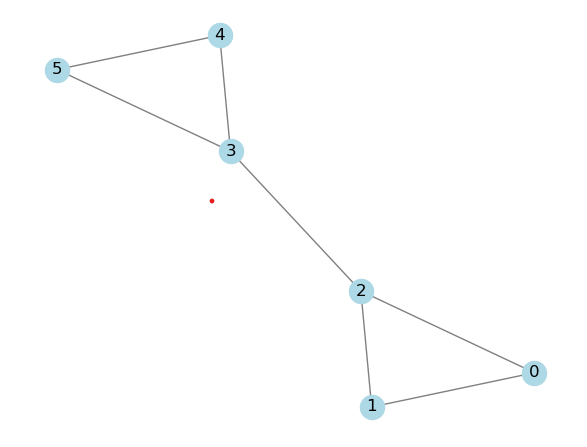
\includegraphics[width=0.3\linewidth]{figures/image00.png} &
$
\begin{bmatrix}
2 & 0 & 0 & 0 & 0 & 0 \\
0 & 2 & 0 & 0 & 0 & 0 \\
0 & 0 & 3 & 0 & 0 & 0 \\
0 & 0 & 0 & 3 & 0 & 0 \\
0 & 0 & 0 & 0 & 2 & 0 \\
0 & 0 & 0 & 0 & 0 & 2 \\
\end{bmatrix}
$ &
$
\begin{bmatrix}
0 & 1 & 1 & 0 & 0 & 0 \\
1 & 0 & 1 & 0 & 0 & 0 \\
1 & 1 & 0 & 1 & 0 & 0 \\
0 & 0 & 1 & 0 & 1 & 1 \\
0 & 0 & 0 & 1 & 0 & 1 \\
0 & 0 & 0 & 1 & 1 & 0 \\
\end{bmatrix}
$ &
$
\begin{bmatrix}
2 & -1 & -1 & 0 & 0 & 0 \\
-1 & 2 & -1 & 0 & 0 & 0 \\
-1 & -1 & 3 & -1 & 0 & 0 \\
0 & 0 & -1 & 3 & -1 & -1 \\
0 & 0 & 0 & -1 & 2 & -1 \\
0 & 0 & 0 & -1 & -1 & 2 \\
\end{bmatrix}
$
\end{tabular}
}
\end{figure}

\vspace{2em}
\noindent\textbf{Example 2: Three-Node Path Graph}

\begin{figure}[h!]
\centering
\resizebox{\textwidth}{!}{
\begin{tabular}{cccc}
\textbf{Graph \(G\)} &
\textbf{Degree Matrix \(D(G)\)} &
\textbf{Adjacency Matrix \(A(G)\)} &
\textbf{Laplacian Matrix \(L = D - A\)} \\
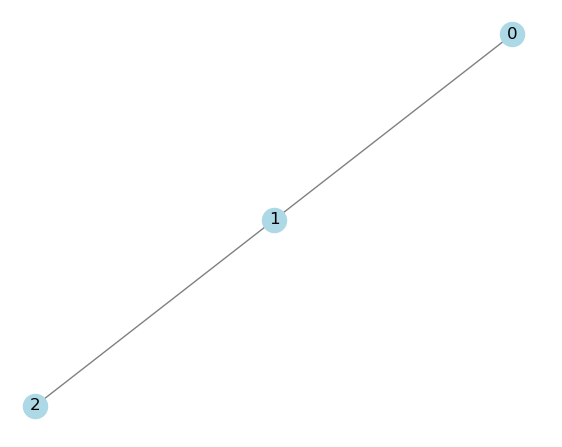
\includegraphics[width=0.2\linewidth]{figures/image03.png} &
$
\begin{bmatrix}
1 & 0 & 0 \\
0 & 2 & 0 \\
0 & 0 & 1 \\
\end{bmatrix}
$ &
$
\begin{bmatrix}
0 & 1 & 0 \\
1 & 0 & 1 \\
0 & 1 & 0 \\
\end{bmatrix}
$ &
$
\begin{bmatrix}
1 & -1 & 0 \\
-1 & 2 & -1 \\
0 & -1 & 1 \\
\end{bmatrix}
$
\end{tabular}
}
\end{figure}

\subsection{Eigenvalues and Eigenvectors of the Laplacian Matrix}
The eigenvalues and eigenvectors of the Laplacian matrix \( L \) provide critical spectral information about the graph's structure.

\begin{itemize}
    \item The eigenvalues \( \lambda \) and eigenvectors \( x \) satisfy the equation:
    \[
    Lx = \lambda x
    \]
    \item The smallest eigenvalue \( \lambda_1 = 0 \), with the corresponding eigenvector being the constant vector (i.e., all entries equal).
    \item The second smallest eigenvalue \( \lambda_2 \) is known as the \textbf{algebraic connectivity} of the graph.
    \item The corresponding eigenvector \( x_2 \) is called the \textbf{Fiedler vector}, which captures how to divide the graph into two parts with minimal edge cuts.
\end{itemize}
%%%%%%%%%%%%%%%%%%%%%%%%%%%%%%%%%%%%%%%%%%%%%%%%
\section{Fiedler’s Spectral Graph Partitioning Method}

\textbf{Fiedler’s method} is a spectral graph partitioning technique that uses the eigenstructure of the Laplacian matrix \( L(G) \) to divide a graph into two subgraphs with minimal edge cuts. It leverages the properties of the \textbf{Fiedler vector}—the eigenvector corresponding to the second-smallest eigenvalue of \( L \).

\subsection{Procedure}
To partition a graph using Fiedler's method, follow these steps:

\begin{enumerate}
    \item Compute the Laplacian matrix \( L(G) = D - A \), where \( D \) is the degree matrix and \( A \) is the adjacency matrix.
    \item Compute the eigenvalues and eigenvectors of \( L(G) \).
    \item Identify the second-smallest eigenvalue \( \lambda_2 \), and extract the corresponding eigenvector \( x_2 \) (the \textbf{Fiedler vector}).
    \item Partition the vertex set \( V \) based on the sign of the entries in \( x_2 \):
    \[
    \text{If } x_i < 0, \text{ assign vertex } i \text{ to } G_1; \quad \text{else assign it to } G_2.
    \]
\end{enumerate}

\noindent \textbf{This approach often produces balanced partitions and reflects the underlying structure of the graph.}

\subsection{Example 1: Six-Node Graph}

\begin{figure}[h!]
\centering

\begin{minipage}[c]{0.33\textwidth}
    \centering

    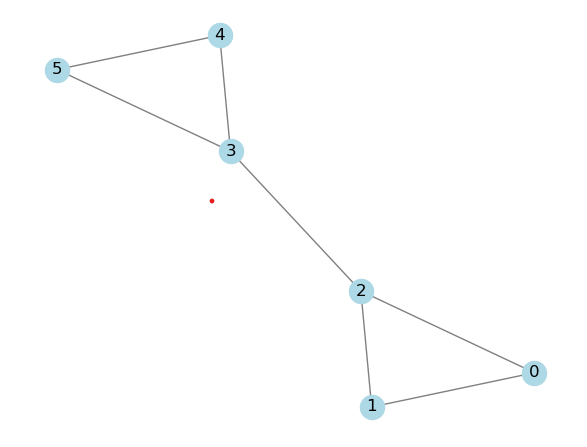
\includegraphics[width=\linewidth]{figures/image00.png}
    \caption*{\textbf{Input Graph}}
\end{minipage}%
\hfill
\begin{minipage}[c]{0.28\textwidth}
    \centering
    \[
    \begin{bmatrix}
    0.4647 \\
    0.4647 \\
    0.2610 \\
    -0.2610 \\
    -0.4647 \\
    -0.4647 \\
    \end{bmatrix}
    \]
    \caption*{\textbf{Fiedler Vector}}
\end{minipage}%
\hfill
\begin{minipage}[c]{0.33\textwidth}
    \centering
    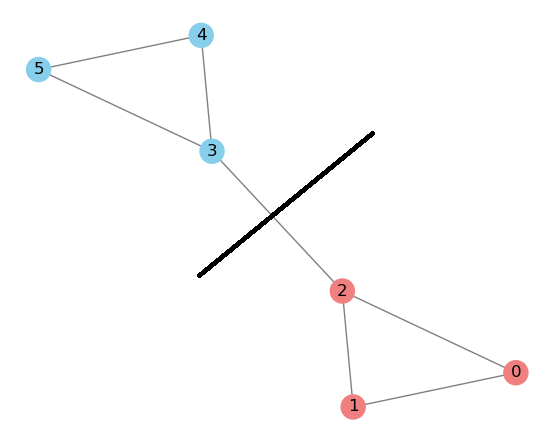
\includegraphics[width=\linewidth]{figures/image01.png}
    \caption*{\textbf{Partitioned Graph}}
\end{minipage}
\end{figure}
\newpage

\subsection{Example 2: Three-Node Path Graph}
\begin{figure}[h!]
\centering
\begin{minipage}[c]{0.33\textwidth}
    \centering
    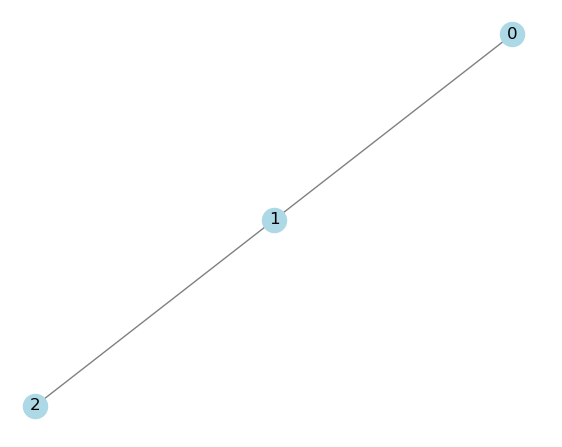
\includegraphics[width=\linewidth]{figures/image03.png}
    \caption*{\textbf{Input Graph}}
\end{minipage}%
\hfill
\begin{minipage}[c]{0.28\textwidth}
    \centering
    \[
    \begin{bmatrix}
    -0.7071 \\
    0.0001 \\
    0.7071 \\
    \end{bmatrix}
    \]
    \caption*{\textbf{Fiedler Vector}}
\end{minipage}%
\hfill
\begin{minipage}[c]{0.33\textwidth}
    \centering
    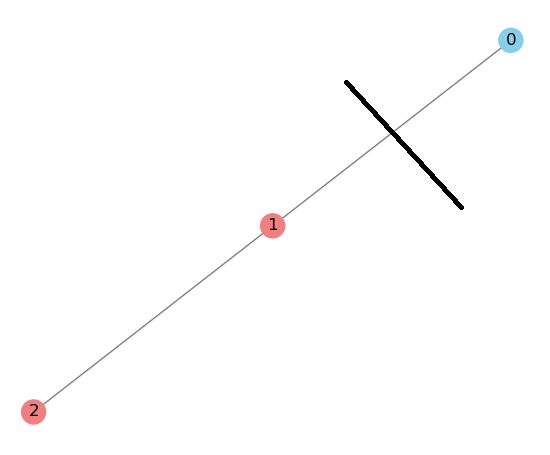
\includegraphics[width=\linewidth]{figures/image04.png}
    \caption*{\textbf{Partitioned Graph}}
\end{minipage}
\end{figure}

\subsection*{Remarks}
While the Fiedler vector provides a natural way to split a graph, the resulting partition is not guaranteed to:
\begin{itemize}
    \item Minimize the total number of edge cuts.
    \item Preserve connectivity within each subgraph \( G_1 \) and \( G_2 \).
\end{itemize}

\noindent Despite this, it is often effective in practice and widely used in applications such as clustering, image segmentation, and load balancing.
%%%%%%%%%%%%%%%%%%%%%%%%%%%%%%%%%%%%%%%%%%%%%%%%%
\newpage
\section{Standing Wave Analogy for Spectral Partitioning}

The connection between Fiedler's spectral partitioning and the theory of vibrating strings provides intuitive insight into why the second eigenvector of the Laplacian—the Fiedler vector—is effective for graph partitioning.

\subsection*{Discrete String Model as a Graph}

Consider a string of length \( L \) fixed at both ends (\( x_0 = 0 \), \( x_{n+1} = L \)), discretized into \( n+1 \) equal segments:

\begin{figure}[h]
    \centering
    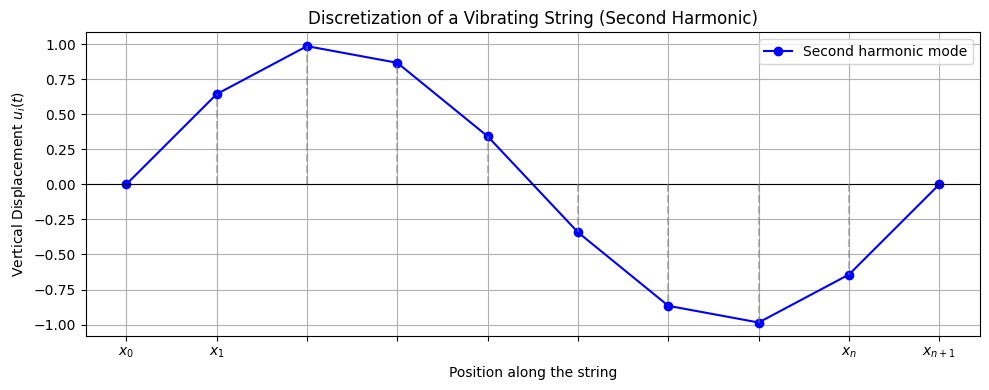
\includegraphics[width=0.7\textwidth]{figures/image02.jpg}
    \caption{Discretized vibrating string showing \( n \) interior points (vertices) connected as a chain graph. The second vibration mode (dashed) naturally partitions the system.}
    \label{fig:string}
\end{figure}

\noindent This system can be modeled as a \textit{chain graph}, where:
\begin{itemize}
    \item Each interior point \( x_i = i \cdot h \) (\( i=1,\dots,n \)) is a vertex.
    \item Edges connect adjacent points.
    \item Segment length \( h = L / (n+1) \) defines spacing.
\end{itemize}

\noindent As \( n \to \infty \) and \( h \to 0 \), this model approximates a continuous string.

\subsection*{Wave Dynamics and the Graph Laplacian}

The vertical displacements \( u_i(t) \) of the discrete string follow a finite-difference version of the wave equation. The system satisfies:
\begin{itemize}
    \item Boundary conditions: \( u_0(t) = u_{n+1}(t) = 0 \)
    \item Displacement vector: \( \mathbf{u}(t) = [u_1(t), \dots, u_n(t)]^T \)
\end{itemize}

\newpage

\noindent Using \textbf{Second Derivative Approximation via Taylor Expansion}:
\begin{align*}
u(x+h) &= u(x) + h u'(x) + \frac{h^2}{2}u''(x) + \frac{h^3}{6}u'''(x) + \mathcal{O}(h^4) \\
u(x-h) &= u(x) - h u'(x) + \frac{h^2}{2}u''(x) - \frac{h^3}{6}u'''(x) + \mathcal{O}(h^4)
\end{align*}

\noindent Adding both:
\[
u(x+h) + u(x-h) = 2u(x) + h^2 u''(x) + \mathcal{O}(h^4)
\quad \Rightarrow \quad
u''(x) \approx \frac{u(x+h) - 2u(x) + u(x-h)}{h^2}
\]


\noindent This finite difference \textbf{leads to a discrete Laplacian Matrix} which is exactly Laplacian matrix of Chain Graph except first and last vertices. 
\[
\frac{d^2 u_i}{dx^2} \approx \frac{u_{i-1} - 2u_i + u_{i+1}}{h^2}
\quad \Rightarrow \quad
L = \frac{1}{h^2}
\begin{bmatrix}
-2 & 1 & & \\
1 & -2 & \ddots & \\
 & \ddots & \ddots & 1 \\
 & & 1 & -2
\end{bmatrix}
\]


\noindent So, the discrete wave equation becomes:
\[
\frac{d^2 \mathbf{u}}{dt^2} = \frac{c^2}{h^2} L \mathbf{u}
\quad \Rightarrow \quad
L \mathbf{v} = -\frac{\omega^2 h^2}{c^2} \mathbf{v}
\]

\noindent This is an eigenvalue problem:
\[
L \mathbf{u} = \lambda \mathbf{u}, \quad \lambda = -\frac{\omega^2 h^2}{c^2}
\]

\noindent For sinusoidal eigenfunctions such as \( f^r = \sin\left(\frac{r \pi x}{L}\right) \), we have:
\[
\lambda = -\frac{4\pi^2 h^2}{c^2} f^r
\]

\subsection*{Eigenvalues of the Discrete Laplacian}

For a chain graph with \( n \) vertices, the eigenvalues of \( L \) are:
\[
\lambda_k = 2\left(1 - \cos\left(\frac{k\pi}{n+1}\right)\right), \quad k = 1,2,\dots,n
\]

\noindent The second smallest eigenvalue (\( \lambda_2 \)) is:
\[
\lambda_2 = 2\left(1 - \cos\left(\frac{2\pi}{n+1}\right)\right)
\]

\noindent The corresponding eigenvector (Fiedler vector) changes sign once and is used to split the graph into two parts.

\noindent We solve for the second natural frequency \( f_2 \) using:
\[
f_2 = \frac{c}{2\pi h} \sqrt{2\left(1 - \cos\left(\frac{2\pi}{n+1}\right)\right)}
\]

\noindent Substitute \( h = \frac{L}{n+1} \):
\[
f_2 = \frac{c(n+1)}{2\pi L} \sqrt{2\left(1 - \cos\left(\frac{2\pi}{n+1}\right)\right)}
\]

\noindent As \( n \to \infty \), apply the Taylor approximation:
\[
\cos\left(\frac{2\pi}{n+1}\right) \approx 1 - \frac{2\pi^2}{(n+1)^2}
\quad \Rightarrow \quad
2\left(1 - \cos\left(\frac{2\pi}{n+1}\right)\right) \approx \frac{4\pi^2}{(n+1)^2}
\]

\noindent So,
\[
f_2 \approx \frac{c(n+1)}{2\pi L} \cdot \frac{2\pi}{n+1} = \frac{c}{L}
\]

\noindent \textbf{Conclusion:} The second vibration mode has frequency \( f_2 = \frac{c}{L} \), which corresponds to the second eigenvalue of the discrete Laplacian and naturally partitions the system.

\subsection*{Generalization to Arbitrary Graphs}

Although derived for a 1D chain, the intuition extends to general graphs:
\begin{itemize}
    \item The Laplacian \( L = D - A \) generalizes the second derivative operator.
    \item The Fiedler vector is analogous to the second standing wave mode.
    \item Spectral partitioning separates the graph at its “weakest” connectivity point, akin to natural vibration nodes.
\end{itemize}

\subsection*{Conclusion from above analogy}

\begin{itemize}
    \item The corresponding frequency \( f \) in the standing wave model equals the second harmonic \( \frac{c}{L} \). In this mode, the particles of the string experience acceleration in opposite directions — half are moving upward, and half downward. This behavior effectively partitions the string into two distinct regions. Analogously, the Fiedler vector partitions a chain graph into two groups of vertices based on the sign of the vector components.

    \item As previously discussed, the second eigenvector of the graph Laplacian \( L(G) \) naturally partitions a chain graph into two nearly equal halves, with the sign change representing the division.

    \item This intuition extends to more complex graphs. In particular, for planar graphs that can be visualized geometrically (e.g., as a trampoline or membrane), the second mode of vibration divides the graph into two balanced regions, much like how a trampoline deforms into two lobes during its second vibrational mode.
\end{itemize}
%%%%%%%%%%%%%%%%%%%%%%%%%%%%%%%%%%%%%%%%%%%%%%%%
\newpage
\section{Spectral Graph Partitioning: Mathematical Proof}

Let \( G = (V, E) \) be an undirected graph with \( n \) vertices. The Laplacian matrix \( L(G) \) is defined as:

\[
L = D - A
\]

where:
\begin{itemize}
    \item \( D \) is the degree matrix—a diagonal matrix where \( D_{ii} = \deg(v_i) \),
    \item \( A \) is the adjacency matrix of the graph.
\end{itemize}

\subsection*{Key Properties of the Laplacian}

\begin{itemize}
    \item \( L \) is symmetric and positive semi-definite.
    \item Its smallest eigenvalue \( \lambda_1 \) is always zero. and associated eigenvector is the constant vector is   \(
    \mathbf{v}_{\lambda_1} = [1, 1, \dots, 1]^T \in \mathbb{R}^{n}.
    \)
\end{itemize}

\subsection*{The Optimization Problem Behind Partitioning}

With \( \lambda_1 = 0 \), the next informative quantity is the second smallest eigenvalue \( \lambda_2 \), known as the \textbf{algebraic connectivity} of the graph.

\noindent The corresponding eigenvector \( \mathbf{x} \in \mathbb{R}^n \), called the Fiedler vector, minimizes the Rayleigh quotient subject to orthogonality to the constant vector:

\[
\lambda_2 = \min_{\mathbf{x} \perp \mathbf{1}} \frac{\mathbf{x}^T L \mathbf{x}}{\mathbf{x}^T \mathbf{x}}.
\]

\noindent Expanding the numerator, we obtain:

\[
\mathbf{x}^T L \mathbf{x} = \sum_{i=1}^n D_{ii} x_i^2 - \sum_{(i,j)\in E} 2x_i x_j
= \sum_{(i,j)\in E} (x_i - x_j)^2.
\]

\noindent This formulation shows that the objective encourages neighboring vertices \( i \) and \( j \) to have similar values, promoting smoothness in the assignment of values over the graph.

\noindent Since \( \mathbf{x} \perp \mathbf{v}_{\lambda_1} \), we have:

\[
\sum_{i=1}^n x_i = 0.
\]

\noindent This constraint ensures that the entries of \( \mathbf{x} \) cannot all have the same sign. Consequently,\textbf{ a natural way to partition the graph is by using the signs} of the components:

\[
V = V_- \cup V_+, \quad \text{where}
\begin{cases}
V_- = \{ v_i \in V \mid x_i < 0 \}, \\
V_+ = \{ v_i \in V \mid x_i \geq 0 \}.
\end{cases}
\]

\noindent Thus, the Fiedler vector yields a bipartition of the graph based on the sign structure of its entries.


\noindent The spectral objective can also be interpreted as:

\[
\lambda_2 = \min_{\sum x_i = 0} \sum_{(i,j) \in E} (x_i - x_j)^2.
\]

\noindent This expression is minimized when adjacent vertices fall on the same side of the partition. When they differ in sign, the squared difference increases the cost—indicating a cut edge.

\noindent Therefore, spectral methods inherently \textbf{ Minimize the number of edges crossing between partitions, and Promote connectivity within partitions.}

\subsubsection*{Balanced Subgraphs}

While the optimization does not explicitly enforce equal-sized partitions, the zero-mean constraint \( \sum x_i = 0 \) often results in approximately balanced subsets. This helps further reduce cross-partition edges, making the cut both small and balanced.

\noindent Spectral graph partitioning thus achieves \textbf{Low edge-cut partitions,and a Balanced vertex sets.} \hfill \(\blacksquare\)

\subsection*{Visual Representation}

\begin{figure}[h!]
    \centering
    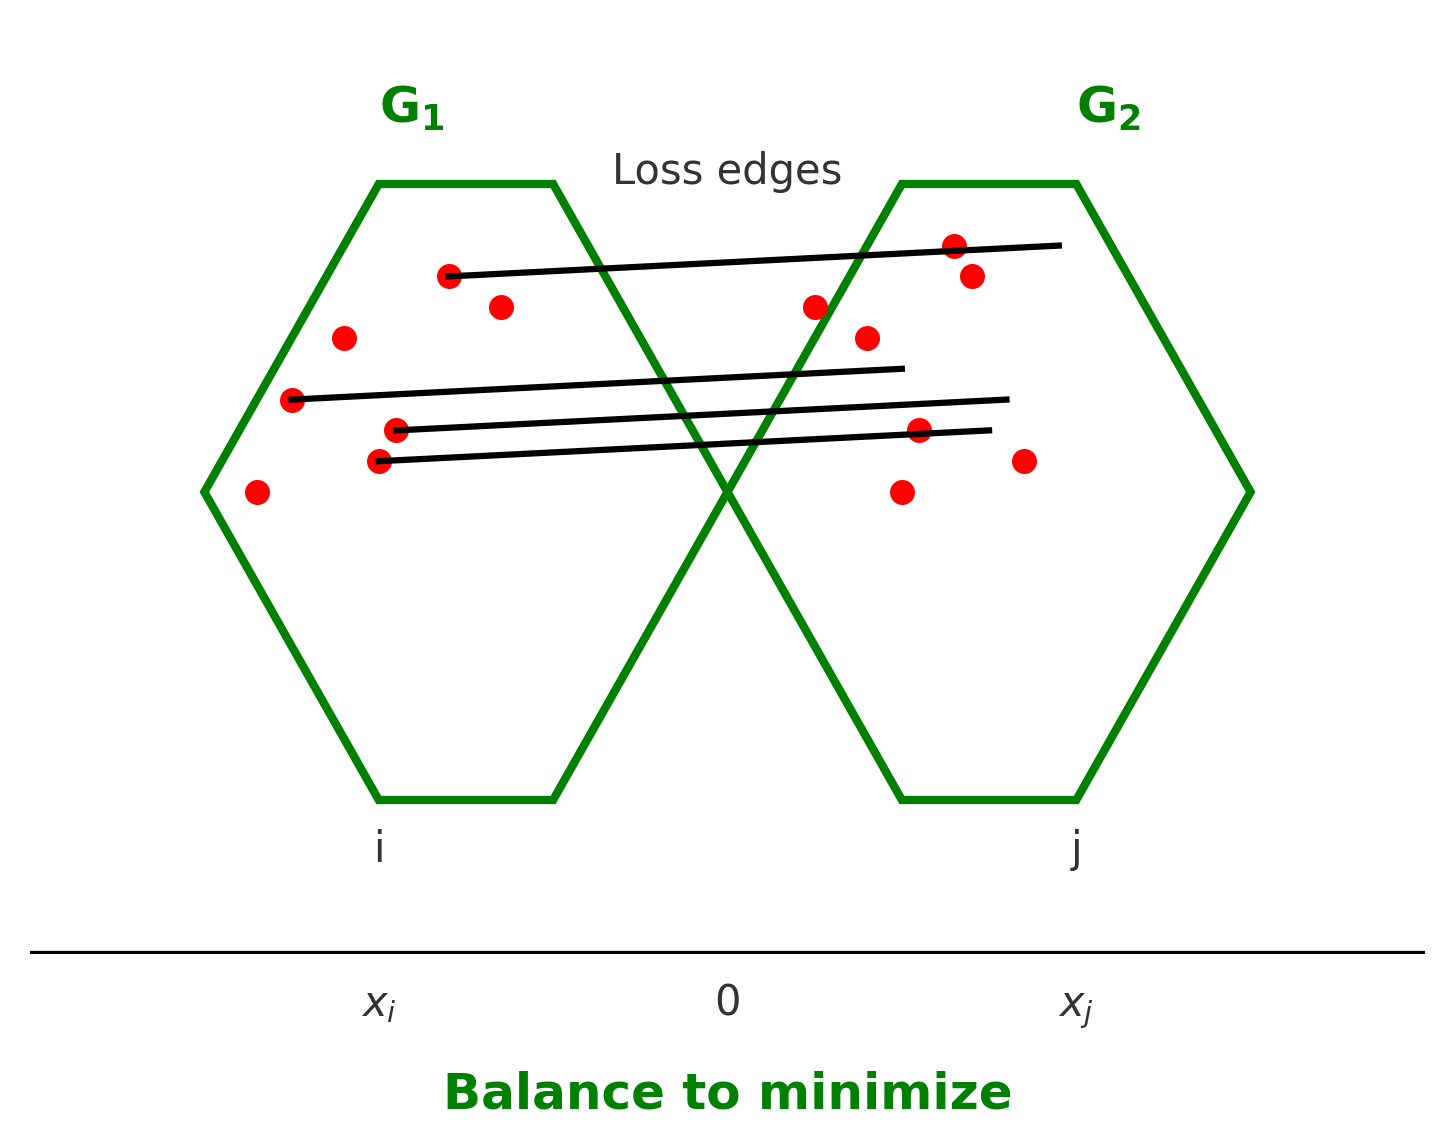
\includegraphics[width=0.7\textwidth]{figures/partition_graph.png}
    \caption{Graph partitioning based on the sign of Fiedler vector components}
    \label{fig:partition_graph}
\end{figure}

\section{Summary of what we did and Next Steps}

\subsubsection*{Established Results:}
\begin{itemize}
    \item A valid graph partition can be derived from the Fiedler vector.
    \item This partition minimizes the number of cut edges.
    \item It tends to produce partitions of approximately equal size.
\end{itemize}

\subsubsection*{Remaining Question:}
We now seek to prove that each subgraph obtained from this spectral partition is \textbf{connected}.

\medskip

\noindent This result stems from a foundational theorem by Miroslav Fiedler, which asserts that partitions induced by the second eigenvector yield connected components under certain conditions.

\medskip

\noindent Before presenting Fiedler’s formal proof, we will build the necessary groundwork by following a simplified and pedagogical path outlined by James Demmel. This involves introducing supporting definitions and lemmas that collectively establish the connectivity of the resulting subgraphs.
\bigskip

\noindent The next section will present these foundational results and then prove the connectivity of the induced subgraphs.
%%%%%%%%%%%%%%%%%%%%%%%%%%%%%%%%%%%%%%%%%%%%%%%
\newpage
\cleardoublepage
\section{Mathematical Preliminaries and Theoretical Foundations}

\subsection{Key Definitions}

\subsubsection*{\textbf{Definition 9.1.1: Non-negative Matrix}}
A matrix \( A \) is said to be non-negative if all of its elements are greater than or equal to zero:
\[
a_{ij} \geq 0 \quad \text{for all } i, j.
\]

\subsubsection*{\textbf{Definition 9.1.2: Spectral Radius}}
The spectral radius of a square matrix \( A \) is the largest absolute value among its eigenvalues:
\[
\rho(A) = \max_{1 \leq i \leq n} |\lambda_i|.
\]

\subsubsection*{\textbf{Definition 9.1.3: Positive Definite Matrix}} 
A matrix \( A \) is positive definite if for all non-zero vectors \( x \), the following holds:
\[
x^\top A x > 0.
\]

\subsection{Remarks}

\subsubsection*{\textbf{Remark 9.2.1: Symmetric and Positive-Definite Matrices}} 
A matrix \( A \) is symmetric and positive definite if and only if every eigenvalue of \( A \) is positive.

\noindent Similarly, \( A \) is symmetric and positive semi-definite if and only if every eigenvalue of \( A \) is non-negative.

\subsection{Lemmas}

\subsubsection*{\textbf{Lemma 9.3.1}}
Let \( A \) be an \( n \times n \) symmetric matrix with eigenvalues \( \lambda_1 \leq \cdots \leq \lambda_n \). Then:
\[
\lambda_1 = \min_{v \neq 0} \frac{v^\top A v}{v^\top v}, \quad \lambda_n = \max_{v \neq 0} \frac{v^\top A v}{v^\top v}.
\]
That is, \( \lambda_1 \) and \( \lambda_n \) are the extremal values of the Rayleigh quotient over all non-zero vectors \( v \in \mathbb{R}^n \).

\noindent \textbf{Proof.} Let \( v \in \mathbb{R}^n \setminus \{0\} \). Define the Rayleigh quotient:
\[
R(v) = \frac{v^\top A v}{v^\top v}.
\]
Let \( y = \frac{v}{\|v\|} \), so \( R(v) = y^\top A y \) with \( \|y\| = 1 \).

\noindent Since \( A \) is symmetric, it is orthogonally diagonalizable: \( A = Q \Lambda Q^\top \), with \( Q \) orthogonal and \( \Lambda = \text{diag}(\lambda_1, \dots, \lambda_n) \). Then:
\[
y^\top A y = (Q^\top y)^\top \Lambda (Q^\top y) = \sum_{i=1}^{n} \lambda_i z_i^2, \quad \text{where } z = Q^\top y \text{ and } \sum z_i^2 = 1.
\]
Thus, \( R(v) \) is a convex combination of the eigenvalues:
\[
\lambda_1 \leq R(v) \leq \lambda_n.
\]
Hence,
\[
\min_{v \neq 0} \frac{v^\top A v}{v^\top v} = \lambda_1, \quad \max_{v \neq 0} \frac{v^\top A v}{v^\top v} = \lambda_n.
\] \hfill \(\blacksquare\)
\vspace{1cm}
\subsubsection*{\textbf{Lemma 9.3.2}} 
Let \( A \) be an \( n \times n \) symmetric matrix. If \( \rho(A) < 1 \), then \( I_n - A \) is nonsingular and:
\[
(I_n - A)^{-1} = \sum_{i=0}^{\infty} A^i.
\]

\noindent \textbf{Proof.}

\noindent \textbf{1. Eigenvalues of \( I_n - A \):}  
Since \( A \) is symmetric, its eigenvalues are real and lie in \( (-1, 1) \). The eigenvalues of \( I_n - A \) are:
\[
\lambda_i(I_n - A) = 1 - \lambda_i(A) \in (0, 2),
\]
so \( I_n - A \) is positive definite and invertible.

\noindent \textbf{2. Convergence of the Series:}  
Diagonalize \( A = Q \Lambda Q^\top \), then:
\[
A^i = Q \Lambda^i Q^\top.
\]
As \( |\lambda_i| < 1 \), \( \Lambda^i \to 0 \), so the series \( \sum_{i=0}^\infty A^i \) converges.

\noindent \textbf{3. Telescoping Sum:}  
Let:
\[
S_m = \sum_{i=0}^{m} A^i.
\]
Then:
\[
(I_n - A) S_m = I_n - A^{m+1}.
\]
As \( m \to \infty \), \( A^{m+1} \to 0 \), so:
\[
(I_n - A) \left( \sum_{i=0}^{\infty} A^i \right) = I_n.
\]
Therefore,
\[
(I_n - A)^{-1} = \sum_{i=0}^{\infty} A^i
\] \hfill \(\blacksquare\)
\newpage
\subsection{Theorems}


\subsubsection*{\large\textbf{Theorem 9.4.1 (Cauchy Interlacing Theorem)}}
Let \( A \in \mathbb{R}^{n \times n} \) be a symmetric matrix with eigenvalues ordered as:
\[
\lambda_1 \leq \lambda_2 \leq \cdots \leq \lambda_n.
\]
Let \( A(i{:}j,\,i{:}j) \) denote the principal submatrix of \( A \), formed by taking rows and columns \( i \) through \( j \), so that:
\[
A(i{:}j,\,i{:}j) \in \mathbb{R}^{(j-i+1) \times (j-i+1)}.
\]
Let the eigenvalues of \( A(i{:}j,\,i{:}j) \) be ordered as:
\[
\chi_1 \leq \chi_2 \leq \cdots \leq \chi_{j-i+1}.
\]

\noindent Then, for any \( k \leq j - i + 1 \), the matrix \( A \) has at least \( k \) eigenvalues less than or equal to \( \chi_k \); that is,
\[
|\{ \lambda_\ell \mid \lambda_\ell \leq \chi_k \}| \geq k.
\]

\subsubsection*{\large\textbf{Theorem 9.4.2}} 

Let \( A \in \mathbb{R}^{n \times n} \) and \( X \in \mathbb{R}^{n \times n} \) be a nonsingular matrix. Then
\[
X^\top A X \text{ is symmetric positive definite } \iff A \text{ is symmetric positive definite}.
\]

\vspace{0.5em}
\noindent \textbf{Proof ( \( \Leftarrow\) direction):} \\
Assume \( A \) is symmetric positive definite, i.e., \( A = A^\top \) and \( \lambda_{\min}(A) > 0 \).
\begin{itemize}
    \item \textbf{Symmetry:} Since \( A = A^\top \), we get \( (X^\top A X)^\top = X^\top A^\top X = X^\top A X \), so \( X^\top A X \) is symmetric.
    \item \textbf{Positive definiteness:} Consider the Rayleigh quotient:
    \[
    \lambda_{\min}(X^\top A X) = \min_{v \ne 0} \frac{v^\top X^\top A X v}{v^\top v}.
    \]
    Let \( y = Xv \), then \( v^\top X^\top A X v = y^\top A y \), and using \( v^\top v = \frac{y^\top y}{v^\top X^\top X v / v^\top v} \), we get:
    \[
    \lambda_{\min}(X^\top A X) \ge \lambda_{\min}(A) \cdot \lambda_{\min}(X^\top X) > 0.
    \]
    Hence, \( X^\top A X \) is positive definite.
\end{itemize}

\newpage
\vspace{0.5em}
\noindent \textbf{Proof ( \( \Rightarrow\) direction):} \\
Assume \( X^\top A X \) is symmetric positive definite.
\begin{itemize}
    \item \textbf{Symmetry:} Since \( (X^\top A X)^\top = X^\top A^\top X = X^\top A X \), we have \( A = A^\top \), so \( A \) is symmetric.
    \item \textbf{Positive definiteness:} As \( X^\top A X \) is positive definite and \( X \) is nonsingular, the Rayleigh quotient gives:
    \[
    \lambda_{\min}(X^\top A X) = \lambda_{\min}(A) \cdot \lambda_{\min}(X^\top X) > 0 \Rightarrow \lambda_{\min}(A) > 0.
    \]
    Thus, \( A \) is positive definite. \hfill \(\blacksquare\)
\end{itemize}
%%%%%%%%%%%%%%%%%%%%%%%%%%%%%%%%%%%%%%%%%%%%%%%
\newpage
\section{Fiedler’s Theorem of Spectral Graph Partitioning}


\subsection*{Theorem and Proof}

\textbf{Fiedler’s Theorem.} \textit{Let $G$ be a connected graph and let $L(G)$ be its Laplacian matrix. Create the subgraphs $G_1$ and $G_2$ using Fiedler’s method (i.e., partitioning based on the sign of the entries in the Fiedler vector). Then, both $G_1$ and $G_2$ are connected.}

\subsubsection*{Proof (by contradiction):}

\begin{itemize}
    \item Assume, without loss of generality, that $G_1$ is disconnected, i.e., it is composed of two connected components.
    
    \item Let $x$ be the eigenvector corresponding to $\lambda_2$, the second-smallest eigenvalue of $L(G)$, also called the Fiedler vector.
    
    \item The Laplacian matrix $L(G)$ and the vector $x$ can be written in block form as:

    \[
    L(G) = 
    \begin{bmatrix}
        L_{1,1} & \mathbf{0} & L_{1,3} \\
        \mathbf{0} & L_{2,2} & L_{2,3} \\
        L_{1,3}^T & L_{2,3}^T & L_{3,3}
    \end{bmatrix}, \quad
    x = 
    \begin{bmatrix}
        x_1 \\
        x_2 \\
        x_3
    \end{bmatrix}
    \]
    
    \item Here:
    \begin{itemize}
        \item $x$ is the Fiedler vector,
        \item $x_1$ and $x_2$ are positive,
        \item $x_3$ is negative.
    \end{itemize}

    \item $O$ denotes matrices of appropriate sizes with all entries equal to zero.
    
    \item Since $L(G)$ is symmetric, all diagonal blocks (e.g., $L_{1,1}$, $L_{2,2}$, $L_{3,3}$) are symmetric matrices, and off-diagonal blocks satisfy $L_{i,j} = L_{j,i}^T$ and are non-positive.
    
    \item Each block $L_{i,j}$ corresponds to the structure of a subgraph or component of $G$.
    
    \item Since the graph is partitioned based on the signs of entries in the Fiedler vector $x$, the vertices corresponding to $x_1$ and $x_2$ are assigned to the same subgraph $G_1$.
    
    \item There are no edges between the vertices corresponding to $x_1$ and $x_2$, since the entries in $L_{1,2}$ and $L_{2,1}$ are zero. This implies that $G_1$ is disconnected, and its components are represented by Laplacian submatrices such as $L_{1,1}$ and $L_{2,2}$.
\end{itemize}
\newpage
\noindent Let $x$ be an eigenvector of $L(G)$ with eigenvalue $\lambda_2$, so:  
\[
L(G)x = \lambda_2 x.
\]

\noindent Consider the first block $x_1$ of $x$. Multiplying out the corresponding block row:  
\[
L_{1,1}x_1 + L_{1,3}x_3 = \lambda_2 x_1.
\]

\noindent Add $\varepsilon x_1$ to both sides:
\[
(\varepsilon I + L_{1,1})x_1 + L_{1,3}x_3 = (\varepsilon + \lambda_2)x_1.
\]

\noindent Since $\varepsilon I + L_{1,1}$ is symmetric positive definite, we use Demmel’s method and let:
\[
\varepsilon I + L_{1,1} = D - N,
\]
where:
\begin{itemize}
    \item $D$ is diagonal,
    \item $-N$ contains off-diagonal entries,
    \item $D^{1/2}$ is the square root of $D$.
\end{itemize}

\noindent Then:
\[
\varepsilon I + L_{1,1} = D^{1/2}(I - M)D^{1/2}, \quad \text{where } M = (D^{1/2})^{-1} N (D^{1/2})^{-1}.
\]

\noindent Since $I - M$ is positive definite, so is \((D-N)\) 
 (From Theorem 9.4.2) and $M$ is symmetric with eigenvalues in $(-1,1)$, Using \textbf{Lemma 9.3.2} we write:
\[
Y = (\varepsilon I + L_{1,1})^{-1} = (D^{1/2})^{-1} \left( \sum_{i=0}^{\infty} M^i \right) (D^{1/2})^{-1}.
\]

\noindent Thus, $Y$ is a nonnegative matrix.

\noindent Multiply the earlier equation by $Y$:
\[
x_1 + Y L_{1,3} x_3 = (\varepsilon + \lambda_2) Y x_1.
\]

\noindent Multiply both sides by $x_1^T$:
\[
x_1^T x_1 + x_1^T Y L_{1,3} x_3 = (\varepsilon + \lambda_2) x_1^T Y x_1.
\]

\noindent by rearranging we get:
\[
(\varepsilon + \lambda_2) \cdot \frac{x_1^T Y x_1}{x_1^T x_1} = 1 + \frac{x_1^T Y L_{1,3} x_3}{x_1^T x_1}.
\]

\noindent Since $x_1^T Y L_{1,3} x_3 > 0$, this implies:
\[
(\varepsilon + \lambda_2) \cdot \lambda_{n_1}(Y) > 1 \Rightarrow \frac{\varepsilon + \lambda_2}{\varepsilon + \lambda_1(L_{1,1})} > 1.
\]

\noindent Hence:
\[
\lambda_1(L_{1,1}) < \lambda_2.
\]

\noindent Similarly, we get:
\[
\lambda_1(L_{2,2}) < \lambda_2.
\]

\noindent Now, consider the block matrix:
\[
B =
\begin{bmatrix}
L_{1,1} & 0 \\
0 & L_{2,2}
\end{bmatrix}
\]

\noindent By the Cauchy Interlacing Theorem(Theorem 9.4.1):
\[
\lambda_2(L(G)) \le \lambda_2(B),
\]
but we showed:
\[
\lambda_1(L_{1,1}), \lambda_1(L_{2,2}) < \lambda_2 \Rightarrow \lambda_2(B) < \lambda_2(L(G)),
\]
a contradiction.

\noindent Therefore, the assumption that $G_1$ is disconnected must be false.

\bigskip
\noindent\textbf{Hence, $G_1$ is connected.}

\noindent\textbf{By symmetry, the same applies to $G_2$. Thus, both $G_1$ and $G_2$ are connected.}
\hfill \(\blacksquare\)

\vspace{8mm}
\noindent Thus, \textbf{Fiedler’s Spectral Partitioning} provides a way to divide a graph into two connected subgraphs with desirable properties. Based on our analysis and demonstrations so far, we have established the following:

\begin{itemize}
  \item The \textbf{Fiedler vector} enables effective partitioning of a graph.
  \item The number of vertices in both subgraphs is approximately balanced.
  \item The partition minimizes the number of edges cut between the two parts.
  \item Each resulting subgraph is \textbf{internally connected}.
\end{itemize}

%%%%%%%%%%%%%%%%%%%%%%%%%%%%%%%%%%%%%%%%%%%%%%%%
\newpage
\section{Implementation : Examples}

All implementations were done using Python. The following examples illustrate spectral graph partitioning using the Laplacian matrix and Fiedler vector.

\subsection*{Example 1}

\begin{figure}[h!]
\centering
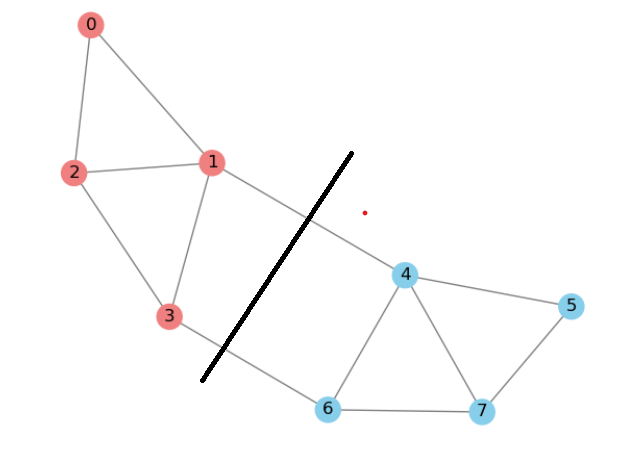
\includegraphics[width=0.5\textwidth]{figures/image06.png}
\caption{Spectral Partitioned Graph for Example 1}
\end{figure}

\noindent\textbf{Laplacian Matrix \(L\):}
\begin{adjustbox}{max width=\textwidth}
\[
\begin{bmatrix}
2 & -1 & 0 & -1 & 0 & 0 & 0 & 0 \\
-1 & 4 & -1 & -1 & -1 & 0 & 0 & 0 \\
0 & -1 & 3 & -1 & 0 & 0 & 0 & -1 \\
-1 & -1 & -1 & 3 & 0 & 0 & 0 & 0 \\
0 & -1 & 0 & 0 & 4 & -1 & -1 & -1 \\
0 & 0 & 0 & 0 & -1 & 2 & -1 & 0 \\
0 & 0 & 0 & 0 & -1 & -1 & 3 & -1 \\
0 & 0 & -1 & 0 & -1 & 0 & -1 & 3 \\
\end{bmatrix}
\]
\end{adjustbox}

\noindent\textbf{Fiedler Vector:}
\[
\begin{bmatrix}
0.4886, 0.2503, 0.1953, 0.4006, -0.2503, -0.4886, -0.4006, -0.1953 
\end{bmatrix}
\]

\noindent\textbf{Lost Edges between \(G_1\) and \(G_2\):} 2
\newpage
\subsection*{Example 2}

\begin{figure}[h!]
\centering
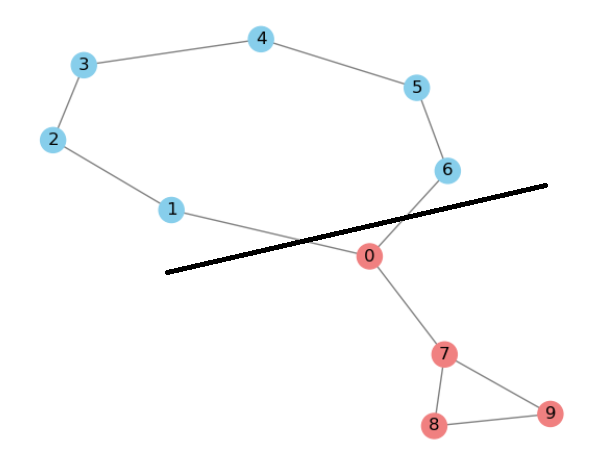
\includegraphics[width=0.5\textwidth]{figures/image05.png}
\caption{Spectral Partitioned Graph for Example 2}
\end{figure}

\noindent\textbf{Laplacian Matrix \(L\):}
\begin{adjustbox}{max width=\textwidth}
\[
\begin{bmatrix}
3 & -1 & 0 & 0 & 0 & 0 & -1 & -1 & 0 & 0 \\
-1 & 2 & -1 & 0 & 0 & 0 & 0  & 0  & 0 & 0 \\
0 & -1 & 2 & -1 & 0 & 0 & 0  & 0  & 0 & 0 \\
0 &  0 & -1 & 2 & -1 & 0 & 0  & 0  & 0 & 0 \\
0 &  0 & 0 & -1 & 2 & -1 & 0  & 0  & 0 & 0 \\
0 &  0 & 0 & 0  & -1 & 2 & -1 & 0  & 0 & 0 \\
-1 &  0 & 0 & 0  & 0  & -1 & 2  & 0  & 0 & 0 \\
-1 &  0 & 0 & 0  & 0  & 0  & 0  & 3  & -1 & -1 \\
0 &  0 & 0 & 0  & 0  & 0  & 0  & -1 & 2  & -1 \\
0 &  0 & 0 & 0  & 0  & 0  & 0  & -1 & -1 & 2 \\
\end{bmatrix}
\]
\end{adjustbox}

\noindent\textbf{Fiedler Vector:}
\[
\begin{bmatrix}
0.0521, -0.1147, -0.2543, -0.3335, -0.3335, -0.2543, -0.1147, 0.3734, 0.4897, 0.4897
\end{bmatrix}
\]

\noindent\textbf{Lost Edges between \(G_1\) and \(G_2\):} 2
\newpage
\subsection*{Example 3}

\begin{figure}[h!]
\centering
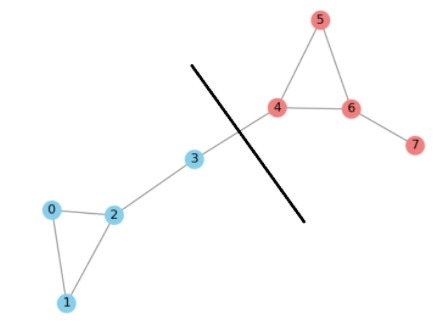
\includegraphics[width=0.5\textwidth]{figures/image10.jpeg}
\caption{Spectral Partitioned Graph for Example 3}
\end{figure}

\noindent\textbf{Laplacian Matrix \(L\):}
\[
\begin{bmatrix}
2 & -1 & -1 &  0 &  0 &  0 &  0 &  0 \\
-1 & 2 & -1 &  0 &  0 &  0 &  0 &  0 \\
-1 & -1 & 3 & -1 &  0 &  0 &  0 &  0 \\
0 &  0 & -1 & 2 & -1 &  0 &  0 &  0 \\
0 &  0 &  0 & -1 & 3 & -1 & -1 &  0 \\
0 &  0 &  0 &  0 & -1 & 2 & -1 &  0 \\
0 &  0 &  0 &  0 & -1 & -1 & 3 & -1 \\
0 &  0 &  0 &  0 &  0 &  0 & -1 & 1 \\
\end{bmatrix}
\]

\noindent\textbf{Fiedler Vector:}
\[
\begin{bmatrix}
-0.4486, -0.4486, -0.3507, -0.0782, 0.2114, 0.3154, 0.3507, 0.4486
\end{bmatrix}
\]

\noindent\textbf{Lost Edges between \(G_1\) and \(G_2\):} 1
\newpage
\subsection*{Example 4}

\begin{figure}[h!]
\centering
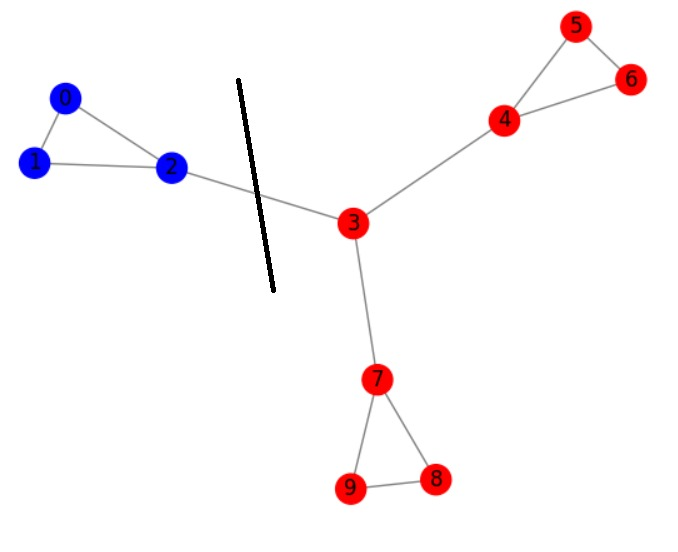
\includegraphics[width=0.4\textwidth]{figures/image11.png}
\caption{Spectral Partitioned Graph for Example 4}
\end{figure}

\noindent\textbf{Laplacian Matrix \(L\):}
\[
\begin{bmatrix}
2 & -1 & -1 &  0 &  0 &  0 &  0 &  0 &  0 &  0 \\
-1 & 2 & -1 &  0 &  0 &  0 &  0 &  0 &  0 &  0 \\
-1 & -1 & 3 & -1 &  0 &  0 &  0 &  0 &  0 &  0 \\
0 & 0 & -1 & 3 & -1 &  0 &  0 & -1 & 0 & 0 \\
0 & 0 & 0 & -1 & 3 & -1 & -1 & 0 & 0 & 0 \\
0 & 0 & 0 & 0 & -1 & 2 & -1 & 0 & 0 & 0 \\
0 & 0 & 0 & 0 & -1 & -1 & 2 & 0 & 0 & 0 \\
0 & 0 & 0 & -1 & 0 & 0 & 0 & 3 & -1 & -1 \\
0 & 0 & 0 & 0 & 0 & 0 & 0 & -1 & 2 & -1 \\
0 & 0 & 0 & 0 & 0 & 0 & 0 & -1 & -1 & 2 \\
\end{bmatrix}
\]

\noindent\textbf{Fiedler Vector:}
\[
\begin{bmatrix}
-0.5127, -0.5127, -0.3753, 0.0000, 0.1877, 0.2564, 0.2564, 0.1877, 0.2564, 0.2564
\end{bmatrix}
\]

\noindent\textbf{Lost Edges between \(G_1\) and \(G_2\):} 1
\newpage
%%%%%%%%%%%%%%%%%%%%%%%%%%%%%%%%%%%%%%%%%%%%%%%%
\section{Limitations of Spectral Partitioning}

Although powerful, spectral partitioning has limitations:

\subsection*{Problematic Cases}

\begin{itemize}
    \item \textbf{Star Graph:} A central node connected to many peripheral nodes. Removing the central edge disconnects the entire graph.
    \item Graphs with highly skewed degree distributions.
    \item Graphs with non-uniform edge density.
\end{itemize}

\subsection*{Reason for Failure}

In such cases, the second smallest eigenvalue (Fiedler value) and its eigenvector may not lead to a meaningful or balanced partition.

\begin{figure}[h!]
\centering
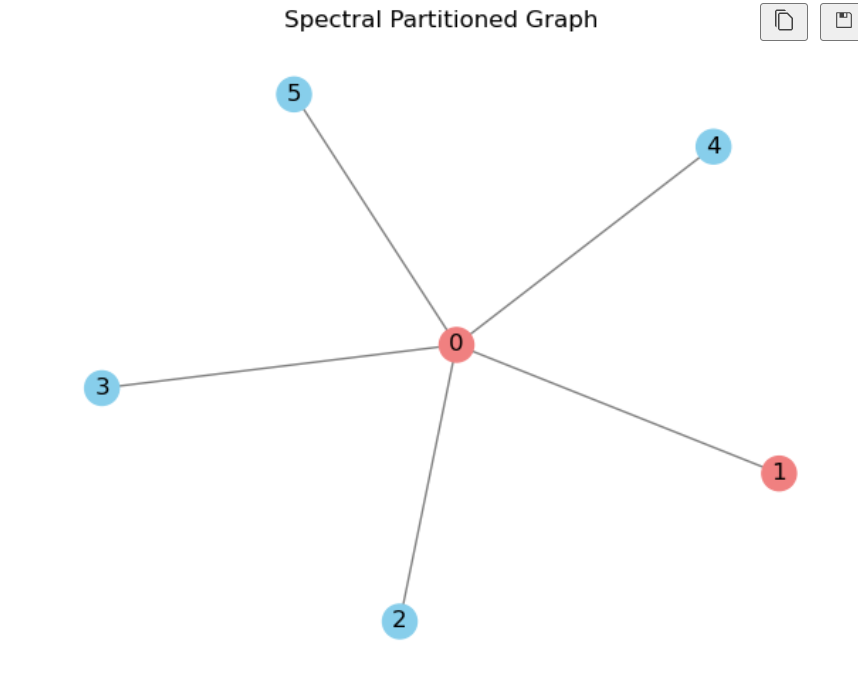
\includegraphics[width=0.5\textwidth]{figures/image09.png}
\caption{Star Graph Example}
\end{figure}
\newpage
%%%%%%%%%%%%%%%%%%%%%%%%%%%%%%%%%%%%%%%%%%%%%%%%
\section*{Industrial Applications}

Spectral partitioning techniques are widely used across various industries due to their ability to identify natural groupings or structures in complex data. Below are some key applications:

\begin{itemize}
    \item \textbf{Community Detection:} Spectral partitioning is used in social network analysis to identify communities or groups of nodes (individuals or organizations) with similar relationships or behaviors. This is crucial for understanding the structure of social networks, detecting influential individuals, and finding tight-knit groups on platforms like Facebook or Twitter.
    
    \item \textbf{Image Segmentation:} In computer vision, spectral partitioning is employed to divide an image into distinct regions with similar properties such as color, texture, or intensity. This technique aids in object recognition, medical imaging, and autonomous vehicle navigation by identifying and separating relevant image regions.
    
    \item \textbf{Web Graph Analysis:} The web is represented as a graph with pages as nodes and hyperlinks as edges. Spectral partitioning techniques help analyze and understand the structure of the internet, aiding in tasks like link prediction, web community detection, and improving search engine optimization (SEO).
    
    \item \textbf{Biological Networks:} In bioinformatics, spectral partitioning is applied to gene or protein interaction networks to uncover functional modules or sub-networks. This helps researchers identify new biological pathways, drug targets, and understand cellular processes at a molecular level.
    
    \item \textbf{VLSI Design:} In very-large-scale integration (VLSI) design, spectral partitioning is used to optimize the layout of circuits on a chip. It minimizes the interconnections between blocks, which results in reduced power consumption, improved chip performance, and faster signal transmission in microprocessors and integrated circuits.
    
    \item \textbf{Parallel Computing:} Spectral partitioning is applied in parallel computing to distribute computational tasks across multiple processors with minimal inter-processor communication. This leads to efficient parallel algorithms and reduces bottlenecks in large-scale scientific simulations or high-performance computing (HPC) environments.
    
    \item \textbf{Recommendation Systems:} In e-commerce and streaming platforms, spectral partitioning helps create personalized recommendations by grouping users with similar preferences. This improves user experience by providing more relevant content, products, or media based on previous behavior.
\end{itemize}
\newpage
\section{Further Work After Fiedler's Decomposition}

Following Fiedler’s decomposition, there are several advanced techniques and methods that can enhance the application of spectral partitioning. These include:

\begin{itemize}
    \item \textbf{Multiway Spectral Clustering:} Instead of just performing a binary partition, multiple eigenvectors can be used to partition a graph into \( k \) clusters. This is particularly useful for problems that involve categorizing data into more than two groups, such as customer segmentation or image categorization.
    
    \item \textbf{Graph Coarsening:} To improve scalability and reduce computational complexity, graph coarsening techniques merge or collapse nodes and edges into supernodes, simplifying the original graph. This approach helps handle large-scale graphs by working with progressively simpler approximations.
    
    \item \textbf{Dynamic Graph Analysis:} Spectral methods can be applied to dynamic or evolving graphs, which change over time. By combining anomaly detection techniques with spectral partitioning, it is possible to monitor shifts in graph structure, such as detecting emerging communities or identifying unusual behavior in social networks or financial markets.
    
    \item \textbf{Spectral Embedding:} Spectral embedding techniques use multiple eigenvectors to map graph nodes into a low-dimensional space (2D or 3D). This visualization aids in understanding complex graph structures, revealing underlying patterns, or providing insights into clustering and community detection in high-dimensional data.
    
    \item \textbf{Graph Signal Processing:} In this advanced technique, the Fiedler vector is treated as a low-frequency signal. It is used for filtering or denoising graph signals, allowing for the extraction of relevant information from noisy or incomplete data. This is particularly valuable in areas like sensor networks or telecommunications.
\end{itemize}
\newpage
%%%%%%%%%%%%%%%%%%%%%%%%%%%%%%%%%%%%%%%%%%%%%%%%

\section{Conclusion}

In this paper, we explored the theory and practical application of \textbf{Spectral Graph Partitioning} using the \textbf{Fiedler vector}. Spectral graph partitioning is a powerful technique for clustering nodes based on graph structure and connectivity. By constructing the graph Laplacian \( L(G) \) from the adjacency and degree matrices, we captured the underlying relationships crucial for effective partitioning. This process is foundational in understanding the behavior of complex networks.
\vspace{3mm}

\noindent A central aspect of spectral partitioning is the second smallest eigenvalue (Fiedler value) and its corresponding eigenvector (Fiedler vector). These components are key for dividing the graph into meaningful clusters, minimizing the edge cut between them. We demonstrated how this technique effectively splits the graph, showing its utility in various applications like community detection and segmentation.
\vspace{3mm}


\noindent The examples provided validated the method's effectiveness, with visually interpretable results. Each partitioned graph was analyzed, and the outcomes from spectral partitioning aligned with intuitive graph structure understanding. The use of visual and matrix-based illustrations helped clarify the algorithm’s logic, making the underlying process easier to follow.
\vspace{3mm}


\noindent Beyond the basic partitioning, further research into spectral methods opens new avenues. These include \textbf{multiway spectral clustering}, using multiple eigenvectors for partitioning into more than two clusters, and \textbf{graph coarsening} to simplify larger graphs for scalability. Additionally, \textbf{dynamic graph analysis} combining anomaly detection with spectral methods can help track graph changes over time, such as in social networks.
\vspace{3mm}


\noindent While spectral partitioning is effective in many cases, it has limitations. Graphs with skewed degree distributions, star-like structures, or non-uniform edge densities can challenge the method. In these cases, the second smallest eigenvalue and eigenvector may not provide meaningful partitions, requiring additional methods or refinements.
\vspace{3mm}


\noindent Spectral partitioning has found wide industrial applications, including \textbf{community detection} in social networks, \textbf{image segmentation} in computer vision, \textbf{VLSI design} for chip layout optimization, and \textbf{biological networks} for identifying gene/protein interaction modules. These applications demonstrate the versatility of spectral methods and their ability to uncover hidden patterns.
\vspace{3mm}


\noindent This work is only the beginning. With the increasing complexity of graphs, further advancements in spectral partitioning are expected. Improvements in algorithmic efficiency and new applications will continue to expand the possibilities for graph analysis in diverse fields.

\newpage
\section{References}

\begin{itemize}
    \item Luxburg, U. von. \textit{A Tutorial on Spectral Clustering}. \textit{Statistics and Computing}, 17(4), 2007. A foundational paper explaining the mathematical principles and practical applications of spectral clustering. Available at: \url{https://doi.org/10.1007/s11222-007-9033-z}
    
    \item Fiedler, M. \textit{Algebraic Connectivity of Graphs}. \textit{Czechoslovak Mathematical Journal}, 23(98), 1973. The original work introducing the Fiedler vector, central to spectral graph theory and partitioning.

    \item Demmel, J. \textit{Graph Partitioning, Part 1}. University of California, Berkeley. Lecture notes covering spectral methods and practical implementation. Available at: \url{http://www.cs.berkeley.edu/~demmel/cs267/lecture18/lecture18.html}

    \item Demmel, J. \textit{Graph Partitioning, Part 2}. University of California, Berkeley. Continuation of the above lecture series with further insights. Available at: \url{http://www.cs.berkeley.edu/~demmel/cs267/lecture20/lecture20.html}

    \item \textit{Fundamentals of Graph Theory} – GeeksforGeeks. A beginner-friendly introduction to graph theory concepts essential for understanding spectral techniques. Available at: \url{https://www.geeksforgeeks.org/fundamentals-of-graph-theory/}

    \item \textit{Spectral Graph Partitioning – Finding a Partition} (YouTube). A visual and intuitive explanation of spectral partitioning with the Fiedler vector. Available at: \url{https://www.youtube.com/watch?v=siCPjpUtE0A&t=1s}
    
    \item \textbf{Supplementary Materials:} All relevant code and resources are available at: \url{https://github.com/AyushmanGHub/Fiedlers-Spectral-Graph-Partitioning-Paper/}
\end{itemize}


%%%%%%%%%%%%%%%%%%%%%%%%%%%%%%%%%%%%%%%%%%%%%%%%
\end{document}
